\chapter{Sentence Translation}
As mentioned previously, training a traditional machine translation system requires large parallel data. With cross-lingual word embedding we can already found ambiguous word translation, in this chapter we propose a simple yet effective method to improve quality of translation which starts from the word-by-word translation. We integrate monolingual model like language model and denoising neural network of the target side to produce meaningful sentence translation. Since all the sub-models  are trained on monolingual corpora, our proposed method is total unsupervised. Our system surpasses state-of-the-art unsupervised translation without costly iteratively training.  
\section{Context-aware Beam Search}
	\subsection{Language Model}
		Language models are widely applied in natural language processing, especially machine translation which need frequent queries. 
		
		${n}$-gram models\\
		${N}$-gram language models use the Markov assumption to break the probability of a sentence into the product of the probability of each word given a limit history of preceding words.
		\[ p(w_1^N) = \prod_{i=1}^{N} p(w_i| w_1, \cdots	w_{i-1}) = \prod_{i=1}^N {p(w_i | w_{i-(n-1)}, \cdots , w_{i-1})}  \] 
		
		The conditional probability can be calculated from ${n}$-gram model frequent counts:
		\[p(w_i | w_{i-(n-1)}, \cdots , w_{i-1}) = \frac{count(w_{i-(n-1)}, \cdots, w_i)}{count(w_{i-(n-1)}, \cdots, w_{i-1})} \]
		Language model tries to handling sparse data problem because some words or phrases have not been seen yet in the training corpus does not mean they are not impossible. Different smoothing techniques like back-off or interpolation are implemented to assign a probability mass to unseen cases.
	\subsection{Beam Search}
	The complexity of a search graph is exponential to the length of the given source sentence. Beam search is a heuristic search algorithm that explores a graph by expanding the most promising nodes. At each step of the search process, it will evaluate all the candidates together with the reserved translation results from last step, it will only stores a predetermined number (beam width) of translations for next step. The greater the beam width is, the fewer states will be pruned. 	
	So it is suggested to prune these word translation candidates as soon as possible to reduce the search space and speed up the translation. According to the similarity of cross-lingual word embedding, we are able to find some meaningful for translation candidates for a given word. But there are also words that actually noise in the candidates or obviously incorrect because of grammar checking. With the support of language model, we can select the most probable words from previous word translation candidates.
	
	Given a history ${h}$ of target word before ${e}$, the score of $e$ to be the translation of ${f}$ is defined as:
	\[ \hat{e}_1^N = \argmax{e_1^N}{\ \prod_{n=1}^{N}} {p^{\lambda_{LM}}(e_n|e_{n-4}^{n-1}) \cdot q^{\lambda_{emb}}(f_n,e_n)}\]

 	where the lexicon score ${q(f,e) \in [0,1]}$ defined as:
 	\[q(f,e) = \frac{d(f,e)+1}{2} \]
 	${d(f,e)\in [-1,1]}$ cosine similarity between ${f}$ and ${e}$
	
	
	In experiments, we find such lexicon score works better than others, e.g. sigmoid or softmax
	
\section{Denoising Neural Network}
\subsection{Denoising Auto-encoder}
	With the help of language model we have actually improved the quality of word-by-word translation but the results are still far from a acceptable one because of the drawback of the word-by-word mechanism, maybe to some degree we can infer the meaning of sentence, but the sequence of sentences depends on the specific language. We implement the sequential denoising autoencoder to improve the translation output.
	
	An autoencoder is a neural network that is trained to copy its input to its output, autoencoders minimize the loss function like: 
	\[ L(\bm x, g(f(\bm x))) \]
	where ${L}$ penalizing the difference between the input and output.
	While a denoising autoencoder (DAE) instead minimizes
	\[ L(\bm x, g(f( \bm {\tilde  x})))\]
	where ${\bm{\tilde{x}}}$ is a noise transformation of ${\bm x}$ and denoising autoencoder will try to learn to ignore the noise in ${\bm x}$ reconstruct the correct one. Sequential denoising autoencoder will find robust representation of sentences.
	In practice,  denoising autoencoder consists of two parts, namely encoder and decoder. The encoder processes noised data and produces real-valued vectors as an encoding feature of the data. The computational graph of the denosing autoencoder, which attempt to reconstruct the normal input ${\bm x}$ from it corrupted version ${\bm{\tilde{x}}}$. The model is trained by minimize the loss.
	
	For our sequential denoising model, the label sequences would be the monolingual data of the target language. However we do not have the noise input. In order to make the model run correctly, we should mimic the noise sentence of word-by-word translation on the target monolingual corpus.
	
	We design different noise types w.r.t. the word-by-word translation. In the experiments, we inject the artificial noise into a clean sentence, the experiment results shows the noise is reasonable and suitable in this case.
	
\subsection{Noise Model}
We design three types of noise to handle the fertility and reordering problem, namely reordering noise, insertion noise and deletion noise. In experiments, the noise model can improve the sentence translation, but since it actually starts from the word-by-word translation, it can only deal with reordering in limited distance, cannot work for global reordering.\\

	\begin{figure}[h]
	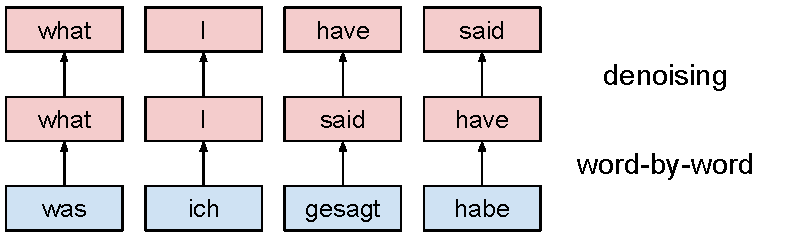
\includegraphics[width=14cm]{denoising}
	\caption{ Reordering noise}
	\centering
\end{figure}
	\textbf{Reordering Noise}\\

	The reordering problem is a common phenomenon in the word-by-word translation since the sequence in source language is not exact the sequence in target language. 
	For example, in  the grammar of German, the verb is often placed at the end of the clause. 
	"um etwas zu tun". However in English it is not the case, the corresponding translation sequence is "to do something". The verb should always before the noun.
	In our beam search, language model only assisting in choosing  more suitable word from the translation candidates, it cannot reorder the word sequence at all.
	
	For a clean sentence from the target monolingual corpora, we corrupt the word sequence by permutation operation. We limit the maximum distance between the original position and its new position.
	
	The design of reordering noise is as followed:
	\begin{enumerate}
		\item For each position ${i}$, sample an integer ${\delta_i}$ from ${[0, d_{per}]}$
		\item Add ${\delta_{i}}$ to index ${i}$ and sort ${i+\delta_{i}}$
		\item Rearrange the words to be in the new positions, to which where indices have been moved
	\end{enumerate}

	Reordering is actually depends on the specific language pair. However in the experiments we found the performance of the denoising network aimed at such noise is not obvious. The Bleu score before and after the process is close.\\

	
	\textbf{Insertion Noise}\\
	\begin{figure}[ht]
	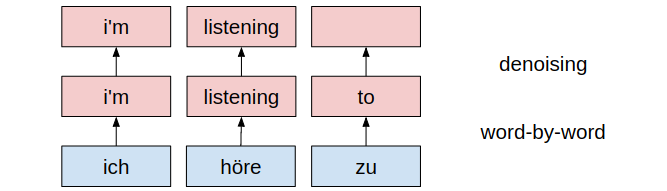
\includegraphics[width=14cm]{insertion}
	\caption{Insertion noise}
	\centering
\end{figure}	

	The word-by-word translation system predict the source word at every position of the sentence. However the vocabularies of different systems are not symmetric, for example, in German there are more compound words than that in English. So when translating cross languages, there are a plenty of cases that a single word will be translated to multiple words and multiple words correspond to a single conversely. We focus on such a case: from a German sentence: "ich höre zu" to "i'm listening". A very frequent word "zu" which corresponds to "to" in English, is dropped from the sentence. The design of reordering noise is as followed:
	\begin{enumerate}	
		\item For each position ${i}$, sample a probability ${p_i \sim \textrm{Uniform}(0,1)}$
		\item If ${p_i} < p_{ins}$, sample a word ${e}$ from the most frequent ${V_{ins}}$ target words and insert it before the position${i}$
	\end{enumerate}

	We limit the insertion word in a set consisting of the top frequent word in the target language ${V_{ins}}$ \\
	
	




	\textbf{Deletion Noise}\\
	The deletion noise is just a contrary case of insertion noise.
	Because we are limited to generate only ne word per source word, it is also possible that a target word in the reference is not related to any source word.  For example for "eine der besten" the corresponding translation is "one of the best". We need to add an extra preposition in the target sentence.  To simulate such situation, we drop some words randomly from a clean target sentence.
	
	\begin{enumerate}
		\item For each position i, sample a probability ${p_i \sim \textrm{Uniform}(0,1)}$
		\item If ${p_i} < p_{del}$, drop the word in the position i
	\end{enumerate}
	
		\begin{figure}[h]
		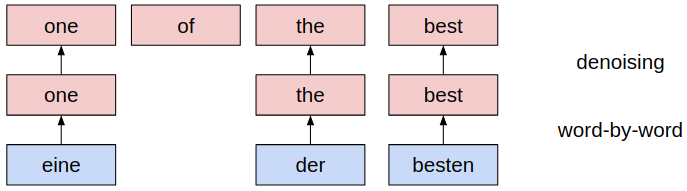
\includegraphics[width=14cm]{deletion}
		\caption{ Deletion noise}
		\centering
	\end{figure}

	
	
	
	
	
	
	
	
	
	
	
	
	
	
	
	
	
	
	
	
	
	
	
	
	
	
	
	